\documentclass[onecolumn, draftclsnofoot,10pt, compsoc]{IEEEtran}
\usepackage{graphicx}
\usepackage{url}
\usepackage{setspace}
\usepackage{graphicx}

\usepackage{geometry}
\geometry{margin = 0.75in}

\title{Writing Assignment One}
\author{Brennan Giles\\CS 444 Oregon State University\\Fall 2018}
\date {24 October 2018}

%%%%%%%%%%%%%%%%%%%%%%%%%%%%%%%%%%%%%%%
\begin{document}
\begin{titlepage}
    \pagenumbering{gobble}
	\maketitle
    \begin{singlespace}
        \begin{abstract}
        % 6. Fill in your abstract    
		In today’s day and age, it is easy to take operating systems for granted. Many don’t understand what they are, and even more don’t think there are any beyond mac and windows. Despite this, entire communities have worked together to create thriving albiet less popular operating systems that often outperform their more famous counterparts. Operating systems like Linux and FreeBSD have the luxury of being able to drop superfluous processes and graphical interfaces in favor of excellent speeds, processes, and security. In this paper, we will examine the advantages and disadvantages of Linux, Windows, and FreeBSD in order to understand their differences and learn more about what makes each Operating system great.
        	
%This document is written using one sentence per line.
%This allows you to have sensible diffs when you use \LaTeX with version control, as well as giving a quick visual test to see if sentences are too short/long.
%If you have questions, ``The Not So Short Guide to LaTeX'' is a great resource (\url{https://tobi.oetiker.ch/lshort/lshort.pdf})
        \end{abstract}     
    \end{singlespace}
\end{titlepage}
\newpage
\pagenumbering{arabic}

\clearpage

% 8. now you write!
\section{Windows Overview}
Windows is an extremely mainstream and widely used operating system that assigns priority to threads instead of processes based on the ascertained importance of those threads. According to the Microsoft Dev Center Manual, “A process has a virtual address space, executable code, open handles to system objects, a security context, a unique process identifier, environment variables, a priority class, minimum and maximum working set sizes, and at least one thread of execution” \cite{WindowsDev}. Windows utilizes CreateProcess in order to create new Processes with process handles. These handles can be passed on to child processes if necessary. CreateProcess also Assigns ProcessID, which can be used to manually access any process through OpenProcess. A more accessable way of seeing and manipulating these processes can be done through “Task Manager”, which displays these processes by name, priority, resource usage, and more. \\

More important to how the kernel operates however are the threads that processes use. “All Threads of a process share its virtual address space and system resources. In addition, each thread maintains exception handlers, a scheduling priority, thread local storage, a unique thread identifier, and a set of structures the system will use to save the thread context until it is scheduled. The Thread context includes the thread’s set of machine registers, the kernel stack, a thread environment block, and a user stack in the address space of the thread’s process” \cite{WindowsDev}. In Windows, preemptive multitasking is supported which allows simultaneous execution of multiple threads from multiple processors, and the system will execute as many threads as possible at the same time. Threads take turns occupying processor time based on priority. Windows processes threads depending on priority and not according to the process the threads are associated with; If process A has 3 threads and process B has 2 then the CPU gives each thread 1/5 of its time as opposed to giving half of its time to A and half to B. \\

	
\section{Linux Overview}
	Linux is the most commonly used operating system in the entire world and according to the IDC dominates the smartphone market as well, controlling over 85 percent of the entire world’s smartphones \cite{IDC}. Linux is a multiprocessing operating system that like windows, strives to use all of the CPU for processes at all times. Each process is represented by a task-struct data structure, and by default the maximum number of processes in the system is limited by the task vector – 512 entries. Processes are kept track of by the "Process ID", or PID. Unlike Windows, processes share lots of information about themselves with eachother such as their state, identifier, links, timers, and more. Processes cannot interrupt other processes and usually run until they need to wait for some sort of system call or exceed their “Time Slice” of usually about 200ms. \cite{tldp} Which process gets to take over next is usually handled by the “Low level scheduler”, which looks for the highest priority thread waiting and runs it. Next, the “high level scheduler” takes over and assigns all the other runnable threads that are still waiting priority. Once assigned priority, these threads are placed in a run queue and the low level scheduler takes over again. \\
	   
	%\texttt{Dynamic real time view of running system accessed through the command "top"} \\
	%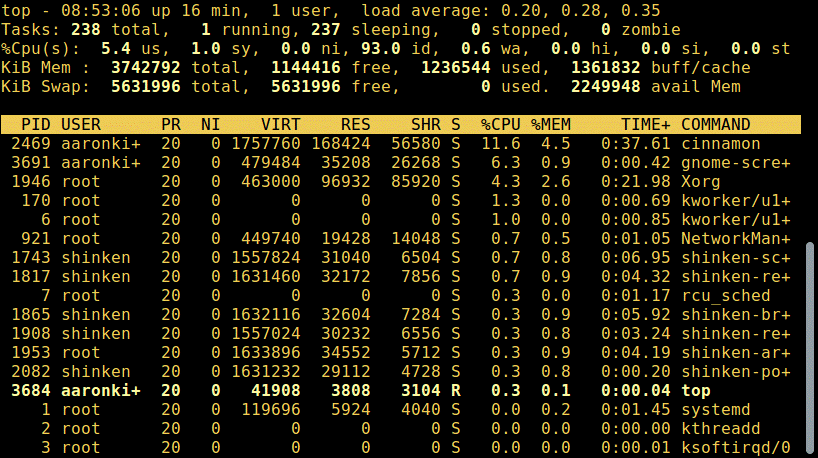
\includegraphics[scale=.5]{top.png} \\
	%\texttt{Courtesy of tecmint.com} \\
	
	Linux is so popular due to its efficiency, adaptability, and simplicity. As stated before, it dominates the smartphone market because it is extremely lightweight; it doesn’t even need a graphical user interface or the bloated features that Windows (10) suffers from. It gets the job done reliably and efficiently and can be configured an infinite amount of ways in order to tailor to any creator’s needs. \\

\section{FreeBSD Overview}
	FreeBSD is an operating system derived from BSD, a version of UNIX developed at the University of California Berkeley. It offers advanced networking, performance, security and compatibility features and does a particularly good job as an internet or intranet server \cite{FreeBSD}. FreeBSD is extremely similar to Linux and shares all the same aspects of process and thread handling. FreeBSD is more commonly used in commercial settings but is available for personal use. Unlike Linux, FreeBSD uses “tcsh” instead of bash as its default shell, which is generally considered not as scripting friendly. One important distinction between Linux and FreeBSD is that Linux is merely a kernel while FreeBSD is an entire Operating system. \\
	
\section{Comparison}
By simply reading the descriptions of each a neat picture of the differences and similarities between the different Systems is made pretty clear, but there are a few more key aspects to discuss. Firstly, closing a parent process in Linux kills all children processes whereas in Windows the children stay alive. Another big difference is that Windows processes don’t share very much information between parent and child while our UNIX friends greatly intertwines the information between the processes. Lastly, Linux in general is considered to have better process handling and creation with fork() compared to windows CreateProcess() based on speed and efficiency. \\

Windows, Linux, and FreeBSD all use priority to choose which processes first, and all use something called “processor affinity” – this enables the binding and unbinding of a process or a thread to a central processing unit (CPU) or a range of CPUs, so that the process or thread will execute only on the designated CPU or CPUs rather than any CPU. \cite{TMurgent} \\

For every job there are different ways to accomplish it, and the same goes for operating systems. Modern technology allows us to exceed in all areas of our lives and it is thanks to the similarities and differences in operating systems that we can choose exactly what we need for success. \\

	
%Bibliography referenced from: https://www.sharelatex.com/learn/Bibliography_management_with_bibtex
\newpage
\begin{thebibliography}{10}
	\bibitem{WindowsDev}
	Windows Dev Center.
	About Processes and Threads
	May 30 2018.
	\\\texttt{https://docs.microsoft.com/en-us/windows/desktop/procthread/about-processes-and-threads}

	\bibitem{IDC}
	Malissa Chau, Ryan Reith, Kathy Nagamine.
	Smartphone OS Marketshare
	October 2 2018.
	\\\textit{https://www.idc.com/promo/smartphone-market-share/os}

	\bibitem{tldp}
    David A. Rusling.
	Chapter 4 - Processes
	September 22 1999.
	\\\texttt{https://www.tldp.org/LDP/tlk/kernel/processes.html}

	\bibitem{FreeBSD}
    The FreeBSD Project.
	About FreeBSD
	January 23, 2018.
	\\\texttt{https://www.freebsd.org/about.html}
	
	\bibitem{TMurgent}
    TMurgent Technologies.
	White Paper - Processor Affinity - Multiple CPU Scheduling
	November 3, 2003
	\\\texttt{http://www.tmurgent.com/appv/en/}


















\end{thebibliography}
\end{document}